% QUESTAO
O valor de $x$ na figura \'e:

\parbox{0.59\linewidth}{

% ALTERNATIVAS
$\sqrt{52+24\sqrt{3}}$
$\sqrt{52+12\sqrt{2}}$
$\sqrt{26+12\sqrt{3}}$
$\sqrt{52}$
$\sqrt{24\sqrt{3}}$

}\parbox{0.4\linewidth}{
\begin{center}
\vspace{-2mm}
\begin{tikzpicture}[rotate=90]
\def\legA{}
\def\legB{}
\def\legC{$150º$}
\triangulo
{$6$}	              {6}	               {0}
{$4$}		  {4}	               {0}
{$x$}	              {9}	               {0}
\end{tikzpicture}
\vspace{-6mm}
\end{center}
}



